%\chapterauthor{Author Name}{Author Affiliation}
%\chapterauthor{Second Author}{Second Author Affiliation}
\chapter{Virtualization and Containerization}

One of the major differences between a server and a personal computer is that the server is usually shared among multiple users at the same time. Though working on the same physical server, a user would usually want a private working environment in the server not interrupted by other users. In other words, each and every user would want to ``virtually'' work on an independent and separated computer with his own CPU, RAM, I/O, OS, drives and hard disk storage, despite that the actual hardware is shared with others. This is done through \textit{Virtualization}, which enables running multiple operating systems on a single physical server in an uninterrupted and logically separated manner. The virtually independent computer of such kind is often called a \textit{virtual machine} (VM).

Deploying a new VM would generally consume considerably large amount of time and computational load, because it needs to load the OS in its first startup. Consider a case where there are hundreds of applications, each requiring running in a similar but separate environment. Launching a VM for each application can be a solution, but it can be expensive due to the time and computational burden. It would be batter to rather deploy only one VM (or physical server) with one OS, and put each application in a ``container'' with its own customized drives and configurations. A container is similar with a VM in the sense that it runs separately from other containers. However, a container is much ``lighter'' than a VM, thus is cheaper to launch and manage. This becomes possible thanks to \textit{containerization}. It is worth mentioning that since a container contains all the configuration and minimum requirement information of the application, running a container on different platforms would generate the same stable result. This is handy when comes to code transferring and cross-platform testing.

The similarity and differences of personal PC, VM, and container applications are summarized in Fig. \ref{chvirtualizationandcontainerization:fig:pcvmcontainersructure}.

\begin{figure}
	\centering
	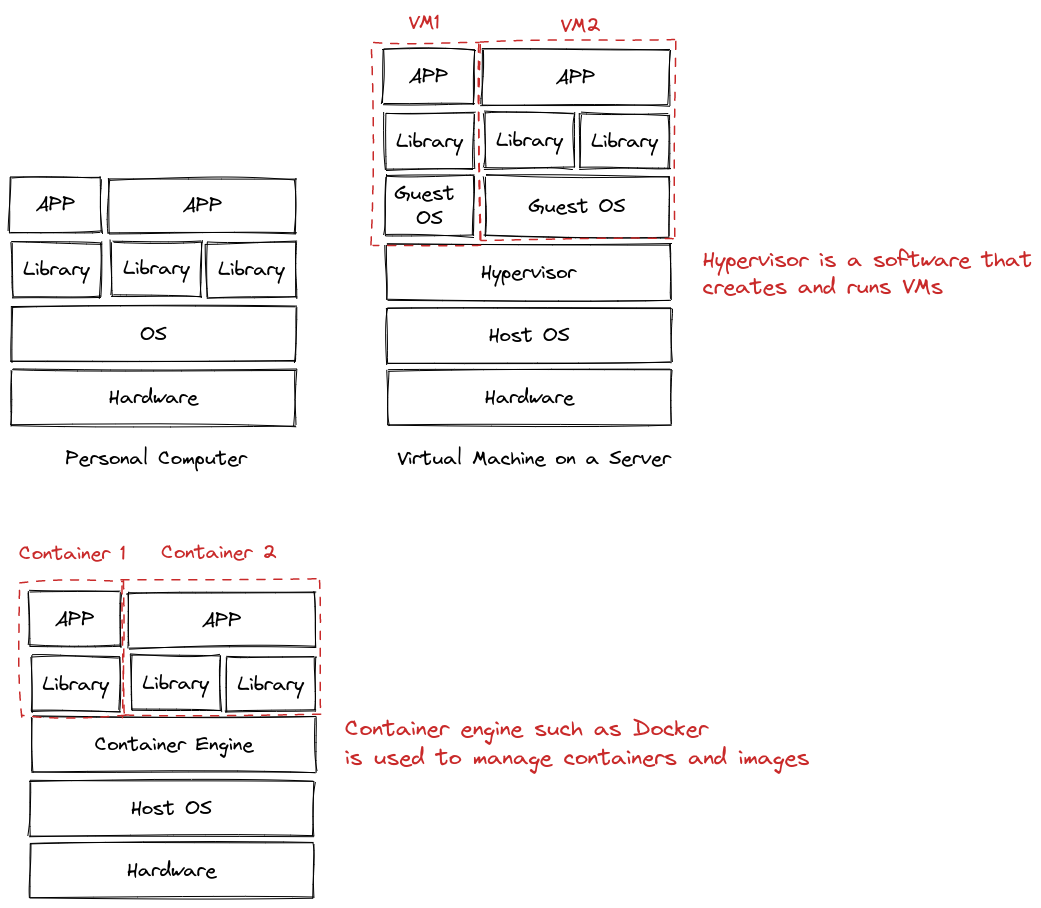
\includegraphics[width=250pt]{chapters/ch_virtualization_and_containerization/figures/pcvmcontainerstructure.png}
	\caption{System architectures of PC, VM and container.} \label{chvirtualizationandcontainerization:fig:pcvmcontainersructure}
\end{figure}

An an analogy, think of running an APP as asking a restaurant to prepare a dish. The hardware is corresponding with kitchen (along with the cooktop, the frying pan, etc.) of the restaurant where every cooking procedure actually happens. The OS is corresponding with the cook, who uses the materials in the kitchen to make the dish. The OS needs associated drivers and libraries to run the APP correctly. The drivers and libraries are like the skill set expected from the cook in order to prepare the dish correctly. Therefore, installing and configuring drivers and libraries in the OS is like teaching the cook new skills (probably from a cookbook) so that he would know how to cook the dish. Finally, the APP is corresponding with the prepared dish.

In a traditional PC implementation, for each customer (user) or dish (APP), a new kitchen is constructed and its associated cook is hired. The cook is trained to master all necessary skills required by the customer or for the dish. A metaphor of the PC implementation is given in Fig. \ref{chvirtualizationandcontainerization:fig:acookinakitchen}.
\begin{figure}
	\centering
	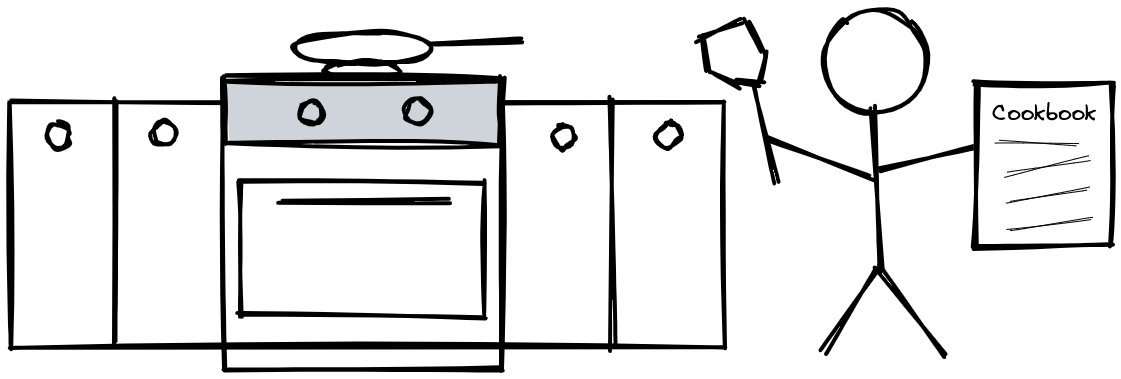
\includegraphics[width=200pt]{chapters/ch_virtualization_and_containerization/figures/acookinakitchen.png}
	\caption{PC implementation: a cook in a kitchen.} \label{chvirtualizationandcontainerization:fig:acookinakitchen}
\end{figure}

In a VM implementation, a larger and more capable kitchen is setup in advance. For each customer or a dish, a cook is hired. Each cook is trained with the skills necessary for his associated customer or dish. All cooks share the same kitchen. This implementation is more efficient than the previous ``a cook in a kitchen'' implementation in Fig. \ref{chvirtualizationandcontainerization:fig:acookinakitchen}, as there is no need to scale up the kitchen for each new customer or APP. By sharing the resources among the cooks, it is more probable that the resources in the kitchen be used more effectively. A metaphor of the VM implementation is given in Fig. \ref{chvirtualizationandcontainerization:fig:manycooksinakitchen}. This is indeed a popular implementation when comes to both enterprise-level server management and a local restaurant.
\begin{figure}
	\centering
	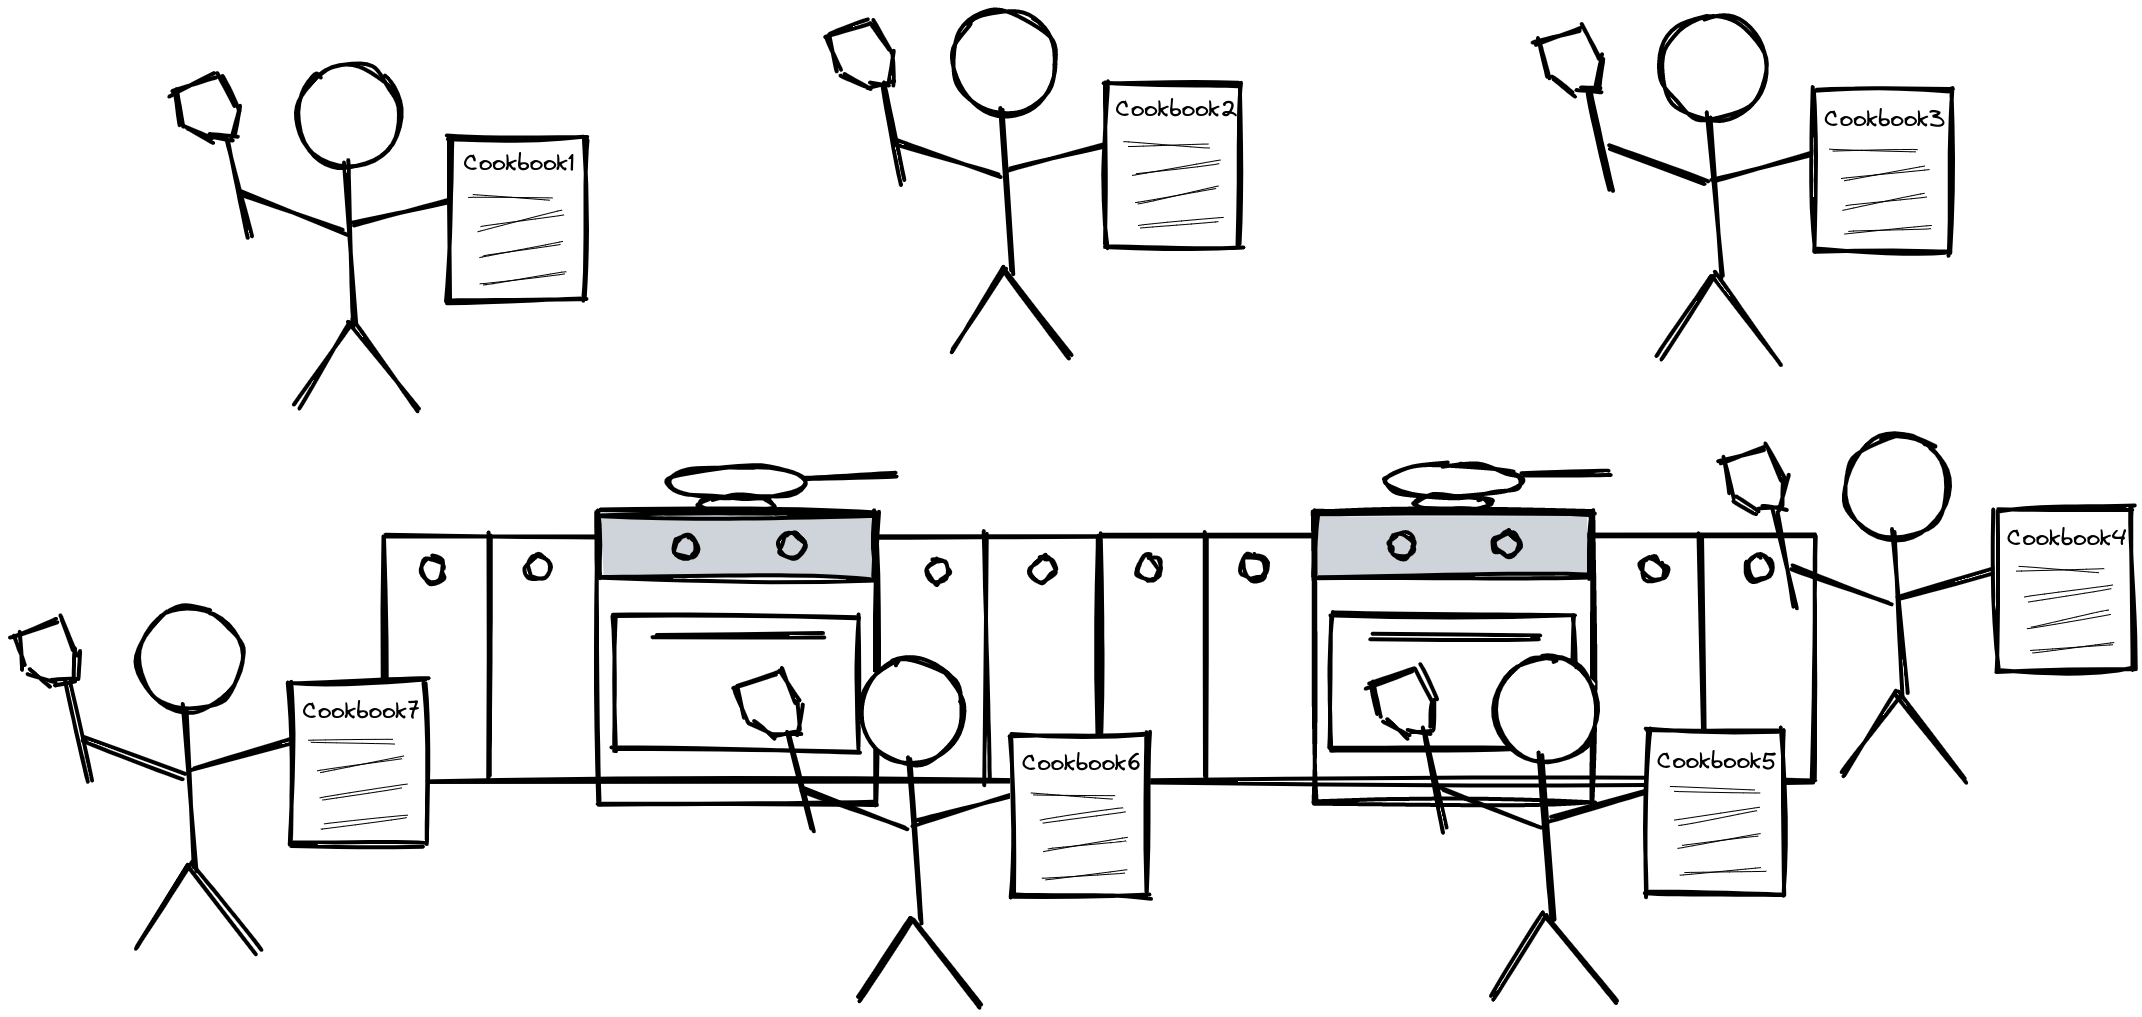
\includegraphics[width=350pt]{chapters/ch_virtualization_and_containerization/figures/manycooksinakitchen.png}
	\caption{VM implementation: many cooks in a kitchen, each with a different cookbook.} \label{chvirtualizationandcontainerization:fig:manycooksinakitchen}
\end{figure}

Deploy dedicated OS for each APP can be time consuming when the number of the APPs is large. This is also true in the restaurant, where it is very rare for each dish to have a dedicated cook. Instead, a cook usually handles a category of dishes that requires similar skill sets. A cook good at multi-task can handle many dishes by himself alone, as long as the dish recipes are provided. Of course, each dish will stay in its own frypan so that they would not affect each other. This is similar with a container implementation. The recipe for a dish, which describes the skill set of the dish, is called an ``image'' of the container that describes the drivers, libraries and basic configurations for the APP to run. The food cooked in the frypan is the APP. The frypan, the food, and the recipe, together form an instance of a container. A metaphor of the container implementation is given in Fig. \ref{chvirtualizationandcontainerization:fig:multitaskcook}. Luckily, the cook (OS) is good at multi-tasking by nature, and with the help of a front desk manager (container management tool such as Docker), he can perform quite well.
\begin{figure}
	\centering
	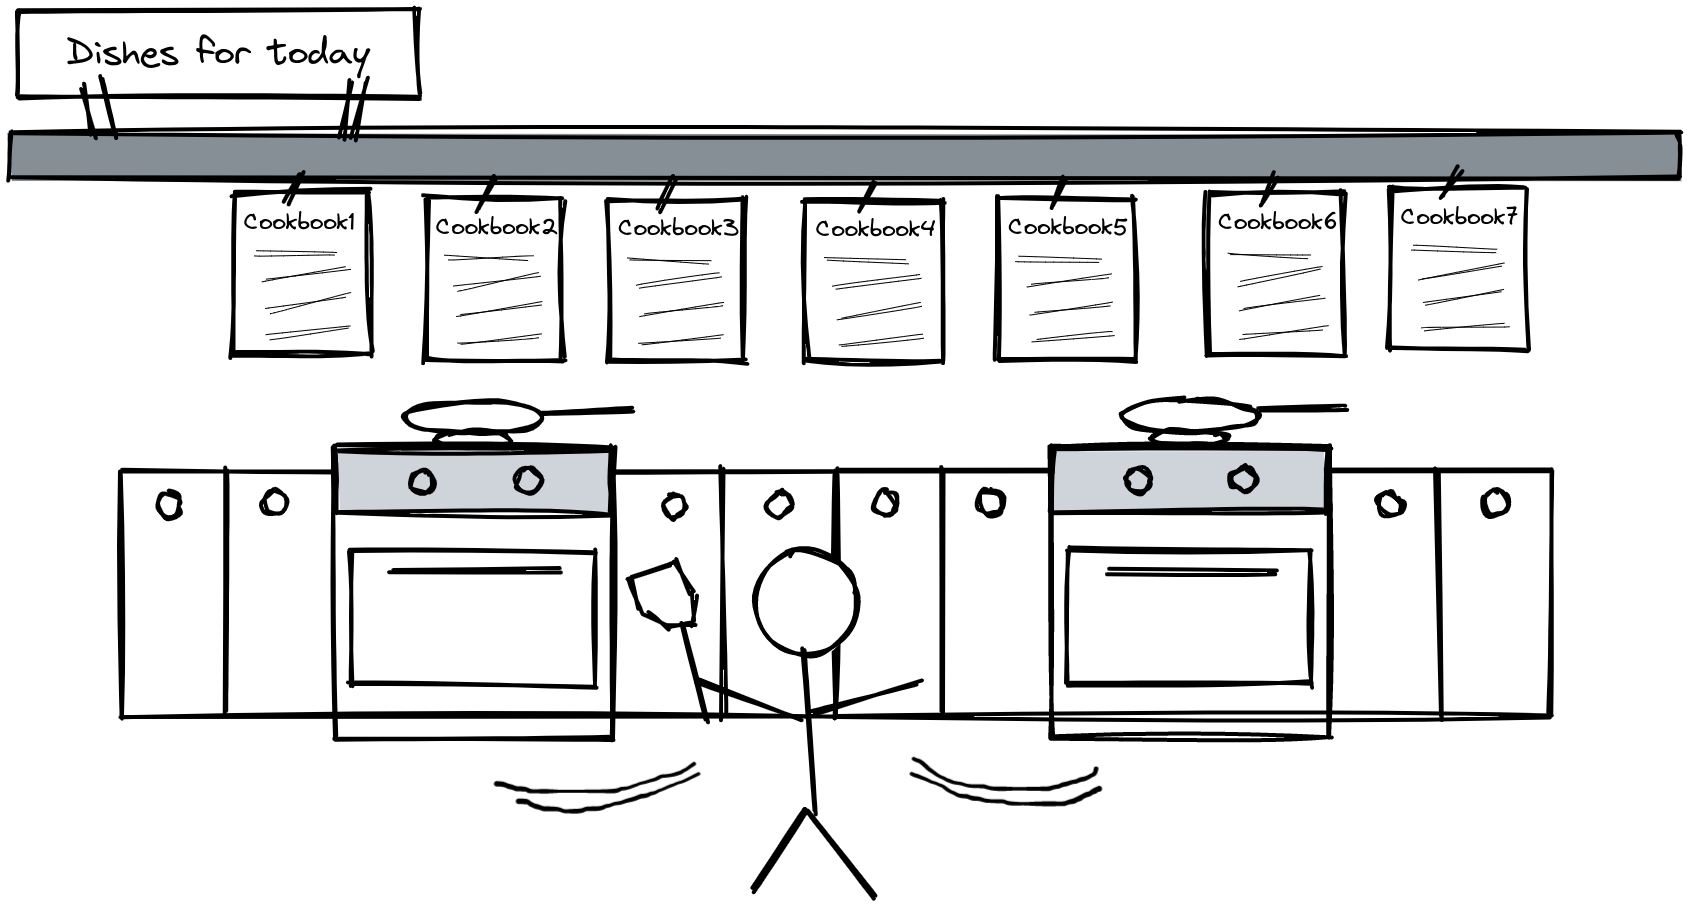
\includegraphics[width=350pt]{chapters/ch_virtualization_and_containerization/figures/multitaskcook.png}
	\caption{Container implementation: one in a kitchen, handling multiple dishes, each has a cookbook and stays in its own pan.} \label{chvirtualizationandcontainerization:fig:multitaskcook}
\end{figure}

A cookbook is a instruction of a dish. It guarantees that the same dish, even one day to be cooked in a different restaurant by a different cook, would taste the same. Similarly, the image of a container serves as the start-up instruction of the container, and it helps to maintain consistency of the performance of the APP even running on different machines between developers and machines, guaranteeing that a APP runs correctly on different machines. With an image, it is convenient to deploy similar container instances quickly.

\section{Virtual Machine}
...
\section{Container}
...
\section{Docker}

\subsection{Docker Installation}

Docker engine is one of the most popular container management engine available online, and it is free of charge for personal non-commercial usage. To install Docker on a Linux machine, go to \textit{https://www.docker.com/} to for the instruction. 

As an example, consider installing Docker engine on Ubuntu. Some of the key steps are summarized as follows.

\vspace{0.1in}
\noindent \textbf{Remove existing Docker engine, if any.}
\begin{lstlisting}
$ sudo apt-get remove docker docker-engine docker.io
$ sudo apt-get remove containerd runc
\end{lstlisting}

\vspace{0.1in}
\noindent \textbf{Add Docker's official GPG key and set up the repository.}
\begin{lstlisting}
$ sudo apt-get update
$ sudo apt-get install ca-certificates curl gnupg lsb-release
$ sudo mkdir -p /etc/apt/keyrings
$ curl -fsSL https://download.docker.com/linux/ubuntu/gpg | sudo gpg --dearmor -o /etc/apt/keyrings/docker.gpg
$ echo \
  "deb [arch=$(dpkg --print-architecture) signed-by=/etc/apt/keyrings/docker.gpg] https://download.docker.com/linux/ubuntu \
  $(lsb_release -cs) stable" | sudo tee /etc/apt/sources.list.d/docker.list > /dev/null
\end{lstlisting}

\vspace{0.1in}
\noindent \textbf{Install Docker.}
\begin{lstlisting}
$ sudo apt-get update
$ sudo apt-get install docker-ce docker-ce-cli containerd.io docker-compose-plugin
\end{lstlisting}

To test whether docker is installed correctly, run 
\begin{lstlisting}
$ sudo docker run hello-world
\end{lstlisting}
and if everything is done correctly, a message started with ``Hello from Docker!'' will be displayed in the console, together with a brief introduction to how docker works.

Notice that to use docker commands, sudo privilege is required. To avoid typing \verb|sudo| each time running a docker command, add the user to the docker group as follows.
\begin{lstlisting}
$ sudo usermod [user_name] -aG docker
\end{lstlisting}

In the rest of the section, \verb|sudo| is neglected for docker commands.

\subsection{Basic Docker Commands}

To run a container from an image, simply use
\begin{lstlisting}
$ docker run [image_name]
\end{lstlisting}
Docker will search the local and remote repository for the image, download the image if necessary, and run the container of that image. By default, after successful execution, the container will go into ``Exited'' status. To customize the container running, for example, assigning a name for the container, flags can be used. Details are introduced later.

To check images stored locally, use
\begin{lstlisting}
$ docker image ls
\end{lstlisting}

To check the status of a container, use
\begin{lstlisting}
$ docker container ls
\end{lstlisting}
or 
\begin{lstlisting}
$ docker container ls -a
\end{lstlisting}
where \verb|-a| indicates displaying both running and exited containers. Without \verb|-a|, exited containers will not be displayed.

For example, consider running a container of \textit{alpine} as follows. A screen shot is given in Fig. \ref{chvirtualizationandcontainerization:fig:dockerrunexp}.
\begin{lstlisting}
$ docker run -it --name test-alpine alpine
\end{lstlisting}
where \verb|-i| stands for interactive, which will keep the container's standard input (i.e., the console in this example) open so that the user can actively interract with the container. Option \verb|-t| allocates a pseudo-TTY to the container, making the interactive interface a bit more user friendly. Finally, \verb|--name| assign a name to the container. Without an assigned name, docker will randomly assign a name to the container.
\begin{figure}
	\centering
	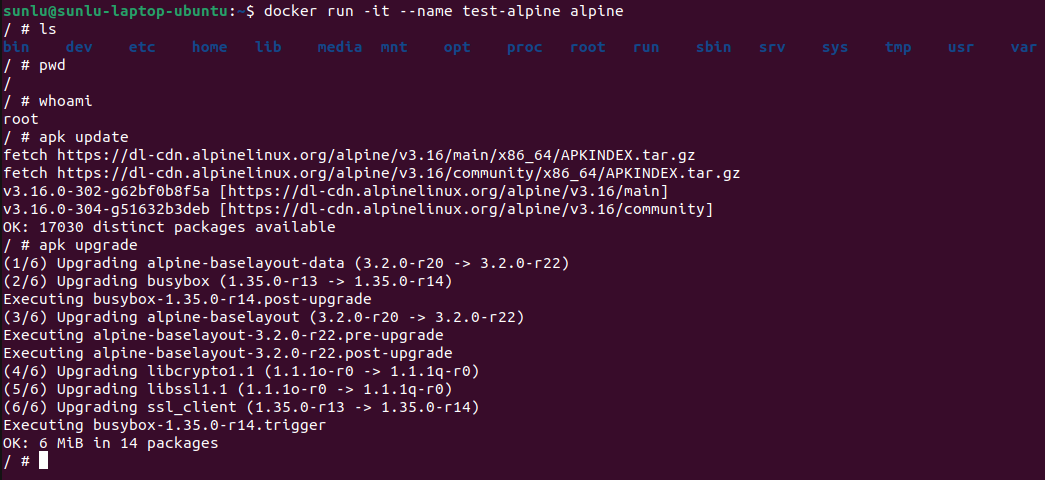
\includegraphics[width=350pt]{chapters/ch_virtualization_and_containerization/figures/dockerrunexp.png}
	\caption{An example of running \textit{apline} container, with interactive TTY and name \textit{test-apline}.} \label{chvirtualizationandcontainerization:fig:dockerrunexp}
\end{figure}

It can be seen from Fig. \ref{chvirtualizationandcontainerization:fig:dockerrunexp} that once the container is started, the user can interact with the container using its shell, and perform actions such as upgrading the container, or deploy a web server, etc. While keep the container up running, open another terminal and use \verb|docker container ls|. The container \verb|test-alpine| shall appear in the list, as shown in Fig. \ref{chvirtualizationandcontainerization:fig:dockerrunexppart2}.
\begin{figure}
	\centering
	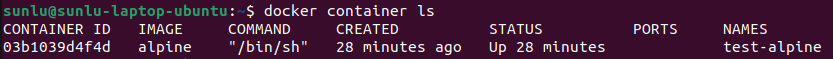
\includegraphics[width=250pt]{chapters/ch_virtualization_and_containerization/figures/dockerrunexppart2.png}
	\caption{List the up running container \textit{test-apline}.} \label{chvirtualizationandcontainerization:fig:dockerrunexppart2}
\end{figure}

If exit from Fig. \ref{chvirtualizationandcontainerization:fig:dockerrunexp} (by using \verb|exit| in the container), the container will transfer its status from up running to exited, as shown in Fig. \ref{chvirtualizationandcontainerization:fig:dockerrunexppart3}.
\begin{figure}
	\centering
	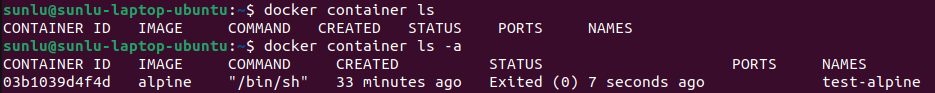
\includegraphics[width=250pt]{chapters/ch_virtualization_and_containerization/figures/dockerrunexppart3.png}
	\caption{List the exited container \textit{test-apline}.} \label{chvirtualizationandcontainerization:fig:dockerrunexppart3}
\end{figure}







